\section{Comparison with database}

A traditional database set up is mostly a client-server type of network architecture. User with the correct log-in credentials and access permissions can query the database and make changes to it. In case of a change to the main database, every user will receive an update next time they access the database. Control of the database remains with database administrators, which allows for access and permissions being maintained by a central authority. Access to the database should be restricted by permissions so only eligible people are able to delete or update information. This works quite differently in a blockchain, in a blockchain, each participant maintains, calculates, updates and validates new entries into the database. All of the participants (nodes) work together to ensure they are all coming to the same conclusions (consensus), providing built-in security for the network. The consequences of this fundamental difference are that blockchains are well-suited as a system of record for certain functions, while a centralised database is entirely appropriate for other functions \cite{steemit}. Almost all blockchains allow different parties that do not necessarily trust each other to share information without requiring a central administrator. 

The contents of a database are stored in the memory and disk of a particular computer system, and anybody with sufficient access to that system can destroy or corrupt the data within. As a result, the moment you entrust your data to a regular database, you also become dependent on the human organisation in which that database resides. Whereas blockchain provides a database that is publicly verifiable and enabled by integrity and transparency: \cite{steemit}
\begin{itemize}
    \item Integrity because every user can be sure that the data they are retrieving is uncorrupted and unaltered since the moment it was recorded.
    \item Transparency because every user can verify how the blockchain has been appended over time.
\end{itemize}


\begin{figure}[H]
    \begin{center}
        \begin{minipage}{\linewidth}
            \begin{center}
                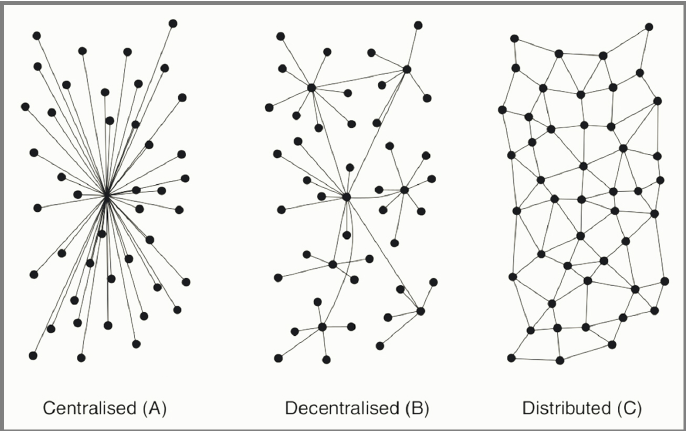
\includegraphics[width=\textwidth,keepaspectratio]{img/centralized-vs-decentralized-vs-distributed-processing.png}
                \caption{Centralized vs decentralized vs distributed processing \cite{cen_dec_dis}}
                \label{obr 1.2.1}
            \end{center}
        \end{minipage}
    \end{center}
\end{figure}

Transparency and integrity are important in elections, where you can't be sure if your vote has been counted or even if your vote was recorded into the database correctly. If an online voting system would be compromised and a person would vote for $X$ your voted could be recorded to the database as $Y$ without your knowledge. In a decentralised solution, the corrupt system would not be trusted and ignored by the network.

\begin{description}
    \item[CRUD vs Read \& Write Operations] In a traditional database, a client can perform four functions on data: Create, Read, Update, and Delete. The blockchain is designed to be append-only structure. A user can only add more data, inform of additional blocks. All previous data is permanently stored and cannot be altered. Therefore, the only operations associated with blockchains are:
    \begin{itemize}
     \item [Read Operations] this query and retrieve data from the blockchain
     \item [Write Operations] these add more data onto the blockchain
    \end{itemize}
    Every blockchain transaction must be digitally signed using a public-private cryptography scheme. This is necessary because transactions propagate between nodes in a peer-to-peer fashion, so their source cannot otherwise be proven. The generation and verification of these signatures are computationally complex and constitutes the primary bottleneck in products like ours. By contrast, in centralized databases, once a connection has been established, there is no need to individually verify every request that comes over it.

    \item[Historical vs Real-time]
    Most central databases keep information that is up-to-date at a particular moment in time, they provide more or less a snapshot of a moment in time but do not provide real-time information. Blockchain databases, on the other hand, are able to keep information that is relevant now, as well as all the information that has come before. Blockchain technology creates a database chain that has a history of itself, they grow as an ever-expanding archive of their own history while providing a real-time portrait. Thanks to their use of cryptography and Merkle trees, the historical information becomes immutable and unchangeable, the only real way to change a blockchain is to add a new transaction that offsets the previous transaction and this can only be done with the consent of all parties involved. The Ethereum hard fork was actually an instance where they reverted to an older state to cancel out a hack of the system; which may have been necessary but an undermining of the principle of blockchain. \cite{steemit2}
    
    \item[Performance] Blockchains as systems of record are considered slow as databases when compared to what is possible for digital transaction technology such as used by Visa and Paypal today. Blockchain technology requires that some speed be sacrificed. The way distributed networks are employed in blockchain technology means that they do not share and compound processing power but rather that they each independently service the network, then compare the results of their work with the rest of the network until there is a consensus that something has happened. Traditional databases, on the other hand, have been around for decades and have seen their performance increase in line with Moore's law.\cite{steemit2}
    
     \item[Robustness]
    A large benefit of blockchain-powered databases is extreme fault tolerance, which stems from their built-in redundancy. Every node processes every transaction, so no individual node is crucial to the database as a whole. Similarly, nodes connect to each other in a dense peer-to-peer fashion, so many communication links can fail before things grind to a halt. The blockchain ensures that nodes which went down can always catch up on transactions they missed. External users can send their transactions to any node, or to multiple nodes simultaneously, and these transactions propagate automatically and seamlessly to everyone else.
    This robustness transforms the economics of database availability. With regular databases, high availability is achieved through a combination of expensive infrastructure and disaster recovery. A primary database runs on high-end hardware which is monitored closely for problems, with transactions replicated to a backup system in a different physical location. If the primary database fails, activity is automatically moved over to the backup, which becomes the new primary. Once the failed system is fixed, it’s lined up to act as the new backup if and when necessary. While all this is doable, it’s expensive and notoriously difficult to get right.

\end{description}

Many of the use cases currently under discussion do not make sense. The biggest problem tends to be confidentiality. The participants in a fiercely competitive marketplace will naturally prefer the privacy of a centralized database, rather than reveal their activities to each other. This is especially true if a trusted central party already exists and can provide the neutral territory in which that database can reside. Even though there may be some cost associated with this central provider, this is more than justified by the value of the privacy retained. The only motivation for a shift to blockchains would be aggressive new regulation. Nonetheless, blockchains do have strong use cases, where disintermediation and robustness are more important than confidentiality and performance. \cite{steemit2}
 